\documentclass[a4paper,12pt]{report}
\addtolength{\oddsidemargin}{-1.cm}
\addtolength{\textwidth}{2cm}
\addtolength{\topmargin}{-2cm}
\addtolength{\textheight}{3.5cm}
\newcommand{\HRule}{\rule{\linewidth}{0.5mm}}
\makeindex

\usepackage{longtable}
\usepackage[pdftex]{graphicx}
\usepackage{makeidx}
\usepackage{hyperref}
\hypersetup{
    colorlinks=true,
    linkcolor=blue,
    filecolor=magenta,      
    urlcolor=cyan,
}


% define the title
\author{Group4_a}
\title{ Assignment 2 Report}
\begin{document}
\setlength{\parskip}{6pt}

% generates the title
\begin{titlepage}

\begin{center}
% Upper part of the page       

\includegraphics[width=1\textwidth]{./up-logo.jpg}\\[0.4cm]    
\textsc{\LARGE Department of Computer Science}\\[1.5cm]
\textsc{\Large COS 301 - Software Engineering}\\[0.5cm]
% Title
\HRule \\[0.4cm]
{ \huge \bfseries COS 301 - Mini Project}\\[0.4cm]
\HRule \\[0.4cm]
% Author and supervisor
\begin{minipage}{0.4\textwidth}
\begin{flushleft} \large
\emph{Author:}\\
Hanrich {Potgieter}
\end{flushleft}
\end{minipage}
\begin{minipage}{0.4\textwidth}
\begin{flushright} \large
\emph{Student number:} \\
u12287343
\end{flushright}
\end{minipage}
\begin{minipage}{0.4\textwidth}
\begin{flushleft} \large
Tshepiso {Magagula}
\end{flushleft}
\end{minipage}
\begin{minipage}{0.4\textwidth}
\begin{flushright} \large
\emph{} \\
u12274195
\end{flushright}
\end{minipage}
\begin{minipage}{0.4\textwidth}
\begin{flushleft} \large
Elana {Kuun}
\end{flushleft}
\end{minipage}
\begin{minipage}{0.4\textwidth}
\begin{flushright} \large
\emph{} \\
u12029522
\end{flushright}
\end{minipage}
\begin{minipage}{0.4\textwidth}
\begin{flushleft} \large
Kruger {Jaco-Louis}
\end{flushleft}
\end{minipage}
\begin{minipage}{0.4\textwidth}
\begin{flushright} \large
\emph{} \\
u13025105
\end{flushright}
\end{minipage}
\begin{minipage}{0.4\textwidth}
\begin{flushleft} \large
Sifiso {Shabangu}
\end{flushleft}
\end{minipage}
\begin{minipage}{0.4\textwidth}
\begin{flushright} \large
\emph{} \\
u12081622
\end{flushright}
\end{minipage}
\begin{minipage}{0.4\textwidth}
\begin{flushleft} \large
Kgomotso {Sito}
\end{flushleft}
\end{minipage}
\begin{minipage}{0.4\textwidth}
\begin{flushright} \large
\emph{} \\
u12243273
\end{flushright}
\end{minipage}
\begin{minipage}{0.4\textwidth}
\begin{flushleft} \large
Neo {Thobejane}
\end{flushleft}
\end{minipage}
\begin{minipage}{0.4\textwidth}
\begin{flushright} \large
\emph{} \\
u11215918
\end{flushright}
\end{minipage}
\begin{minipage}{0.4\textwidth}
\begin{flushleft} \large
Michael {Nunes}
\end{flushleft}
\end{minipage}
\begin{minipage}{0.4\textwidth}
\begin{flushright} \large
\emph{} \\
u12104592
\end{flushright}
\end{minipage}
\vfill
% Bottom of the page
{\large \today}
\end{center}
\end{titlepage}
\footnotesize
%\input{declaration_of_originality.tex}
\normalsize

\renewcommand{\thesection}{\arabic{section}}
\newpage
\begin{center}
\textsc{\LARGE Architecture requirements}\\[1.5cm]
\textsc{\Large Buzz Space Discussions/Mini Project}\\[0.5cm]
Version: Version 0.2 Alpha 
For further references see \href{ https://github.com/MichaelNunes/Cos301-phase-2-group-4-a}{gitHub}.
\today
\end{center}
\tableofcontents{}
For further references see \href{https://github.com/MichaelNunes/Cos301-phase-2-group-4-a}{gitHub} or got to the link https://github.com/MichaelNunes/Cos301-phase-2-group-4-a

\section{Architecture requirements}
\subsection{Access channel requirements}
	Access channel requirements
The buzz space should not only be accessible via desktop/laptop based web browsers, but also mobile devices.

Mobile devices include, but are not restricted to cell phones and tablets. In general mobile devices refers to devices with a fairly smaller screen than a laptop or PC, but can also be carried around with ease. 

Mobile devices allow users to contribute and collaborate on the buzz spaces wherever they go. In order to ensure ease of use for mobile users, the site should adapt accordingly.

Rendering of a mobile version of the website should thus be required in order to maximise ease of use for mobile users. Since a mobile app will not be developed, mobile sites should be of high importance when designing the website. The mobile websites does not need to be an entire different site, such as a .mobi website, where the main website would be for example .co.za. The need for a responsive website therefore arises.
 
The main website should cater for large screen sizes (PC and laptops), medium screen sizes (tablets) and smaller screen sizes (mobile phones.) This can be achieved by making use of 3 different breakpoints as well as media-queries. The different breakpoints will then ensure that the page is rendered differently according to the various screen sizes. 

The website should also ensure maximum utilisation of enabled technologies on mobile devices. If it is assumed that most of the users will have smartphones, this will however not be an issue, as most smartphone devices support JavaScript, CSS3 and HTML 5, as these are the main components of a modern responsive website. If the cell phone of the client does however not support JavaScript, a website without certain client side functionality should be rendered.

The site should however also be accessible via different systems, not only accessed by users and their web browser enabled devices. It should also be able to integrate the website into other existing systems. This should be enabled by making use of iframes, but this is not recommended due to safety issues. The site should therefore be accessible by making use of hyperlinks to reach the entry point of the buzz spaces.

\subsection{Quality Requirements}
	%\documentclass[a4paper,12pt]{report}
%\addtolength{\textwidth}{2cm}
%\addtolength{\topmargin}{-2cm}
%\addtolength{\textheight}{3.5cm}
%\newcommand{\HRule}{\rule{\linewidth}{0.5mm}}

%\begin{document}

\begin{itemize}
	\item \textbf{Scalability}
		There is a anticipated increase in entry volume. We are expecting an exponential increase in students using the system. It is predicted that this year 750 students are registered for COS132 by next year there will be close to a thousand. We expect a 25 percent growth rate over the next two years. The system must scale and incorporate with the standard Computer Science website. 
	\item \textbf{Performance Requirements}
		Security, web portal and personalised applications will access the the directory server. They will performe various functions such as file access and Database access.
	\item \textbf{Maintanability}
		The system will be comprise of modules and using a Singleton design pattern to handle communication. Thus a centralised node that all communication will pass through between modules. This will allow us the easily edit/add/remove modules from the system.
		\begin{itemize}
			\item \textbf{Documentation}
				Using UML to keep source code organised. Automatic generation of classes.
			\item \textbf{Application Architecture Standards}
				Multilayer design compliance.
		\end{itemize}
	\item \textbf{Reliability and Availability}
		Reliability will definitely be a priority. We will use a server that guarantees us at least 99 per uptime. This will probably be a University of pretoria server. Apply java OO and structured programming practices.
	\item \textbf{Security}
		Clients must not have file access to the server and the root assess of the system must only be allowed to authorised personal. Designing strong password policies and using \textbf{security methods}.
		\begin{itemize}
			\item Authentication
			\item Encryption
			\item Access control
			\item Auditing
		\end{itemize}
	\item \textbf{Monitorability and Auditability}
		The server logs will allow us to monitor the system. These will be provided to us by the systems reporting module. Linux server logs will also allow us to audit the system and monitor its state.
	\item \textbf{Testability}
		Each function will be tested. But mathematical proofs for correctness is not necessary. Each part of the system must be tested. 
	\item \textbf{Usability}
		The web pages must be usable and follow a responsive design approach. This means the pages will display correctly on each screen size. We will follow google material design standards to ensure responsiveness.
	\item \textbf{Integrability}
		The system must be able to integrate into an existing computer science website. We must meet their standards when it comes to obtaining user information. We will conform to all communication standards to the system. Also provide our own integration library which will gain access through out singleton node.
\end{itemize}

%\end{document}
\subsection{Integration requirements}
	
\subsubsection{Channels}
\begin{itemize}
\item REST: Representational State Transfer
\begin{itemize}
\item The REST architecture design is a good option to use as it is a simpler than SOAP and is a dynamic design.
\item A RESTul system can integrate well with HTTP as RESTful systems are optimized for the web.
\item Restful systems needs to follow a client-server model,so this means that there needs to be communication between the client and server which is vital in the buzz system.
\item There is support for a lot of components to interact with each other and to be interchangeable.
\end{itemize}
\end{itemize}
\subsubsection{Protocols}
\begin{itemize}
\item Http(Hypertext Transfer Protocol) is the main protocol for all websites in the modern internet usage.It allows linking of nodes which allows the users to easily navigate through web pages.
\item HTTPS is a more secure version of Http.HTTPS is a combination of HTTP and TSL and SSH.This protocol will ensure that data is safely transported.
\item TCP/IP(Transfer Communication Protocol/Internet Protocal) Used to as communication over the internet.TCP is reliable and is able to check for errors in the transfer of the page over the IP.
\item SMTP(Simple Mail Transfer Protocol) is used to send emails.This will be easier then mailing manually and is prominently used in the web space.
\item IPv6(Internet Protocol version 6) This will  redirected and to allow them to be redirect users or routed to the correct space on the internet.This provides access to buzz through the use of http and the TCP/IP protocols.
\item IPsec(Internet Protocol Security) will allow for a secure IP and to ensure no harmful data is ever transmitted to the servers of buzz.
\end{itemize}

\subsubsection{API Specifications}
\begin{itemize}
\item WSDL - WSDL will be used to describe the functionality and the operations provided by the web-based service (Buzz system).
\item CORBA - CORBA will mediate the communication between the diverse systems that will be integrated to the Buzz system to provide added functionality and data for the operation of the system.
\item IDL - This will be used for data analysis purposes for the data passed from the data source to the Buzz system and any other form of data required by the system.
\end{itemize}

\subsubsection{Integration Quality Requirements}


Integration Approach
The ideal Integration approach that will cater for the needs of the Buzz system is the Document-based Integration because only essential data that is required by the system will be provided by the data source.

The following requirements need to be fulfilled to ensure optimal operation of the system after integration:
\begin{itemize}

\item Performance - The integration should not impact poorly on the performance of the Buzz system. The data required should be easily accessible at all times when requested by the system without compromising the Buzz systems ability to evaluate user credentials or any functionality that is dependent on the data source.
\item Scalability - The data source will contain a large volume of records pertaining to the students registered for the module making use of the Buzz system and therefore has to have the capability to handle a large data set and multiple concurrent users.
\item Reliability - When the Buzz system requires certain records in an efficient timely manner, reliability is also a major concern. To allow proper accessibility, functionality and productivity of the system, reliable data has to be delivered at all times or else the whole system will not operate as desired.
\item Security - The data provided will come from a reliable data source that has sensitive information regarding students who are registered and the details of the system itself. During the integration process, the Buzz system cannot compromise the data source by feeding malicious data to intentionally or unintentionally extract valuable information. The Buzz system can only access records that the data source deems as essential for the use of the Buzz system.
\item Auditability - Every request that is passed by the Buzz system for sensitive data has to be evaluated and assessed to determine whether or not the Buzz system has the rights to obtain that data. Certain requested have to be logged if they produce certain errors or faults in the system that could compromise any of the quality requirements.
\end{itemize}
\subsection{Architecture constraints}
	%\documentclass{article}
 
%\begin{document}

	\begin{enumerate}
		\item Database technology: 
		\item Programming paradigm: 
		\item Programming language: 
		\item Development platform:  
		\item System architecture: 
		\item Architectural frameworks: 
		\item Architectural patterns: 
		\item Development technologies:
		\item IDE:NedBeans
		\item Build environment:
		\item Web server software:
		\item Web interface protocol:
		\item Client web browser:
		\item Client device operating systems:
		\item Source control management: 
		\item Text encoding: UTF-8
		
		
			\subsection{System architecture}
				Layered reference architecture will be used as it is enforced in the JAVA-EE framework
				
			\subsection{Time Constraint }		
					Given 2 weeks for the functional requirements, 1 week for the architectural requirements, 4 weeks 							for the implementation of the system and 1 week for testing.	
					
		
			\subsection{Web services}		
				REST access channel will be used as is more lightweight and doesn’t require a lot of bandwidth, this 						enhances the goal of one of the core quality requirements which is accessibility to many students, 					thus they can access via phone device web browsers with easy.
				
				\subsection{Environmental Constraints}
					The system will be deployed at the University of Pretoria computer sciences server as an 									improvement to the current discussion board system.
					
					\subsection{Authentications}
					LDAP will be used for login authentication as the system is constraint to the University of 									Pretoria Students and already the Department have been using LDAP.
					
					\subsection{Database Technology}
					MySQL will be used as it enhances scalability , is open source ,thus will not cost university that 					much and have features for security that includes serialization, encrypting of passwords ,hashing 						and many more which can be implemented for strengthen security to the system.

		
					
				
				
	\end{enumerate}

%\end{document}

\section{Architectural patterns or styles}
	
\begin{figure}[H]	
\graphicspath{ {images/} }
    	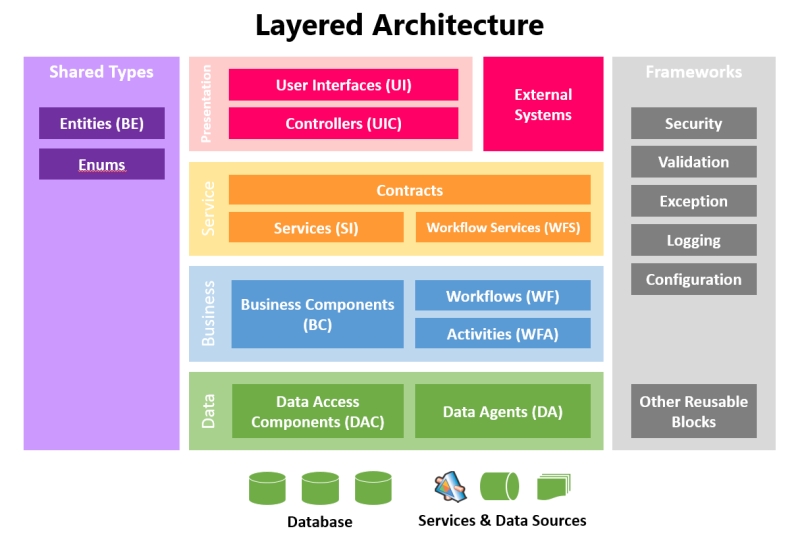
\includegraphics[scale=0.5]{layered.png}
    	\caption{Layered Architecture }
	\end{figure}
\subsection*{Layered Architecture}

System will be separated through layers; there will be User Interface  layer, services layer and process layer which includes Business logic and data. User Interface layer will handle interaction like receiving input from users, the service layer will provide the human layer with services like opening a buzz space and commenting on the buzz thread and lastly process layer will process services rendered for authorization and quality check like plagiarism. Separation through layers will enhance performance, manageability and reusability.

\begin{figure}[H]	
\graphicspath{ {images/} }
    	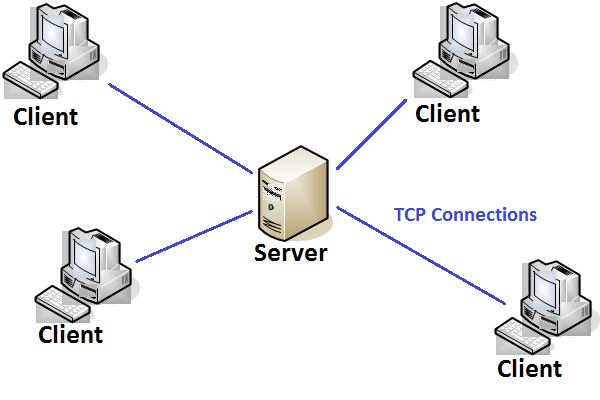
\includegraphics[scale=0.5]{csp.png}
    	\caption{Client/Server}
	\end{figure}
	
\subsection*{Client/Server} 
For communication of the server which is buzz system with users, this pattern have benefits of security as all data will be stored on the buzz system server and ease of maintenance as server is responsible of repair with client knowing of damage.


\subsection*{Model-View-Controller (MVC)}

\begin{flushleft}

Adhering to the MVC design pattern provides us with numerous benefits:

\begin{enumerate}
	\item \textbf{Separation of design concerns:} Because of the decoupling of presentation, control, and data persistence and behavior, the application becomes more flexible; modifications to one component have minimal impact on other components.
	\item \textbf{More easily maintainable and extensible:} Good structure can reduce code complexity. As such, code duplication is minimized.
	\item \textbf{Promotes division of labour:}Developers with different skill sets are able to focus on their core skills and collaborate through clearly defined interfaces.
\end{enumerate}

	\begin{figure}[H]
		\centering\graphicspath{ {images/} }
		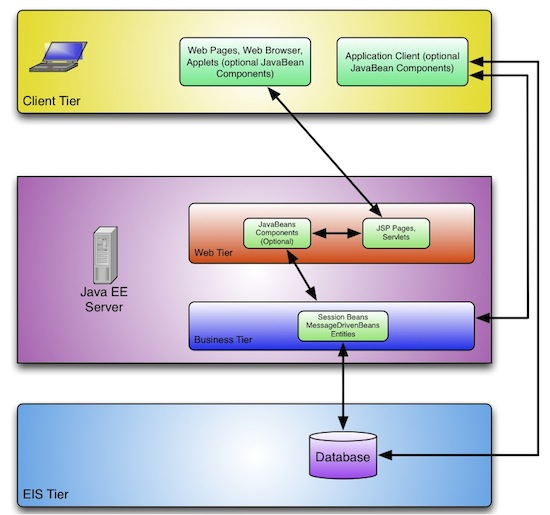
\includegraphics[width=\textwidth, height=15cm]{MVC.jpg}
	   	\caption{Java-EE system architecture}.
	\end{figure}

The system will be designed using the MVC architectural pattern combined
with a multi-tier/layered architectural pattern to form what is known as the Java-EE system architecture.
This will allows the user to be decoupled from the server and the view, the controller and the model each 
to have their own set of layers as described below.

\textbf{View (Client Tier)}\\
This tier runs on the user system and encapsulates the various components that a user system may use to access the Java EE server-side tiers. These components include dynamic web pages, Java applications and Java applets. 

\textbf{Controller (Java-EE server)}

The middle tier's business functions handle client requests and process application data, storing it in a permanent data store in the data tier.

\begin{itemize}
	\item \textbf{Web Tier}
	\\The web tier consists of components that handle the interaction between clients and the business tier.
	
	\item \textbf{Business Tier}
	\\The business tier consists of components that provide the business logic for an application. Business logic is code that provides functionality to a particular business domain.
\end{itemize}

\textbf{Model (Enterprise Information Systems (EIS) Tier)}\\
The EIS tier consists of database servers, enterprise resource planning systems, and other legacy data sources. These resources typically are located on a separate machine than the Java EE server, and are accessed by components on the business tier.

\end{flushleft}

\subsection*{Dependency Injection}

\begin{flushleft}

Dependency injection implements inversion of control for software libraries, where the caller delegates to an external framework the control flow of discovering and importing a service or software module.\\
The benefits of using Dependancy Injection in our system, is that it will ensure loose coupling of code between the different modules that need to be implemented. Decoupling of code will ensure that the code in the system are cleaner, easier to modify when required and easier to adapt and implement for reuse. Dependancy injection also enables the creation of new objects that make use of dependancies.
\end{flushleft}



\section{Architectural tactics or strategies}
	In this section discuss any architectural tactics or strategies you are using to concretely address any
of the quality requirements.
For example, you could be using thread pooling and/or caching to achieve a higher level of
scalability or performance.
Discuss how the strategy is realized within your software architecture.
\section{Use of reference architectures and frameworks}
	\subsubsection{Reference Architecture}

The type of reference architecture that will be used is a Layered reference architecture and therefore 
Java-EE is the Layered reference architecture best suited for the Buzz system. Java-EE is the best choice
because it encompasses most of the quality requirements that we want to exploit which are scalability, security,
reliability and integrability.
\section{Access and integration channels}
	Clients will access the system by using mobile phones, tablets or desktops to log in through a web browser. Therefore HTTPS requests from web browsers will access the systemís services. LDAP will also be used to access student information that is stored in a database on a server. Java EE, Apache Server, HTTPS and Java Persistence API will be used for these actions.
\section{Technologies}
	We will be using JAVA as our main programming language. The server will be running on a linux operating system. The database will be MySQL but object orientated. To build our projects we will use MARVEN.

% Workin with references
% here we add our citations	
\begin{thebibliography}{9}
\bibitem{classRepMeeting}
  Prof Andries Engelbrecht,
  \emph{Class Represetative Meeting}.
	University Of Pretoria,
	Wednesday, 4 March 2015,
	IT Building, room 4-66,
  	2015.
\end{thebibliography}
\end{document}
